%%%%%%%%%%%%%%%%%%%%%%%%%%%%%%%%%%%%%%%%%%%%%%%%%%%%%%%%%%%%%%%%%%%%%%
%% Numerical Techniques
%% (C) Kenneth Geisshirt (kneth@chem.ruc.dk)
%% Last modified: 8 January 1998
%%%%%%%%%%%%%%%%%%%%%%%%%%%%%%%%%%%%%%%%%%%%%%%%%%%%%%%%%%%%%%%%%%%%%%

\chapter{Numerical Techniques}
\label{chap:NumTech}

The results presented in the present thesis are based upon numerical
simulations. The simulational techniques used are the ``experimental
setup'' which has been used. All simulation programs which have been
designed and implemented, are of the Molecular Dynamics (MD) type. This
chapter describes the MD techniques.

The core of the chapter is about soft particles \ie systems where the
particles interact through a smooth potential. The simulation of hard
spheres are discussed in section \ref{sect:HardSpheres}.

In the last decade a number of monographs on computer
simulations has been published. Allen \etal \cite{Allen87} have written
the most well-known and cited monograph. It is 
now a bit out-of-date. While the monograph by Allen \etal dealt with
both Molecular Dynamics and Monte Carlo techniques, the book by
Rapaport \cite{Rapaport95} is considering MD only. Smith \etal
\cite{Smit96} have recently written a book about molecular simulations,
and it is more focused on the physics behind the simulations while
Rapaport is more concerned with the algorithms.


\section{Naive algorithm}
\label{sect:Naive}
In chapter \ref{chap:Mech} classical mechanics was discussed. The
naive idea behind Molecular Dynamics is to solve the equations of
motion of $N$ particles \ie it is a numerical technique which enable
us to solve 

\begin{subequations}
\label{NT:eom}
  \begin{eqnarray}
    \diff{\vec{r}_i}{t} &=& \vec{v}_i  \label{NT:eomA}\\
    \diff{\vec{v}_i}{t} &=& \frac{\vec{F}_i}{m_i}
    \label{NT:eomB}
  \end{eqnarray}
\end{subequations}
where $\vec{r}_i$ is the position of particle $i$, $\vec{v}_i$ the
velocity, $\vec{F}_i$ the force, and $m_i$ the mass. We will assume
that the force is pairwise additive \ie

\begin{equation}
  \vec{F}_i = \sum_{j=1}^{N} \vec{F}_{ij}
\end{equation}
where $\vec{F}_{ij}$ is the force between particle $i$ and $j$. 

The naive algorithm is:

\begin{algorithm}
  \caption[A naive MD program]{A naive MD program}
  \label{prg:NaiveMD}
  \begin{algorithmic}
    \FOR[$M$ is the number of time steps]{$i=1$ to $M$}%
      \STATE \texttt{CalcForce}($\vec{r}_1, \ldots, \vec{r}_N$, 
             $\vec{F}_1, \ldots, \vec{F}_N$)
      \STATE \texttt{Integrate}($\vec{r}_1, \ldots, \vec{r}_N$, 
             $\vec{v}_1, \ldots, \vec{v}_N$, 
             $\vec{F}_1, \ldots, \vec{F}_N$)
    \ENDFOR
  \end{algorithmic}
\end{algorithm}

where the two procedures \texttt{CalcForce} and \texttt{Integrate} are
given as algorithm \ref{prg:NaiveCalcForce} and algorithm
\ref{prg:NaiveIntegrate}, respectively.

\begin{algorithm}
  \caption[A naive force calculation]{A naive force calculation algorithm, \texttt{CalcForce}}
  \label{prg:NaiveCalcForce}
  \begin{algorithmic}
    \REQUIRE $\vec{r}_1, \ldots, \vec{r}_N$, $\vec{F}_1, \ldots,
    \vec{F}_N$
    \FOR{$i=1$ to $N$}
      \STATE $\vec{F}_i \leftarrow \vec{O}$ 
    \ENDFOR
    \FOR{$i=1$ to $N$}
      \FOR{$j=1$ to $N$}
        \STATE $\vec{F}_i \leftarrow \vec{F}_i +
  \vec{F}_{ij}(\vec{r}_i, \vec{r}_j)$
      \ENDFOR
    \ENDFOR
  \end{algorithmic}
\end{algorithm}


\begin{algorithm}
  \caption[A naive integrator]{A naive integration algorithm, \texttt{Integrate}}
  \label{prg:NaiveIntegrate}
  \begin{algorithmic}
    \REQUIRE $\vec{r}_1, \ldots, \vec{r}_N$, $\vec{v}_1, \ldots,
    \vec{v}_N$, $\vec{F}_1, \ldots, \vec{F}_N$
    \FOR[$h$ is the length of the time step]{$i=1$ to $N$}
      \STATE $\vec{v}_i \leftarrow \vec{v}_i +
             h\times\frac{1}{m_i}\vec{F}_i$
      \STATE $\vec{r}_i \leftarrow \vec{r}_i + h\times\vec{v}_i$
    \ENDFOR
  \end{algorithmic} 
\end{algorithm}

In algorithm \ref{prg:NaiveIntegrate} the equations of motion are
solved in a very primitive way. We have approximated the derivatives
by the well-known approximation

\begin{equation}
  \diff{y}{x} \approx \frac{y(x+h) - y(x)}{h}
\end{equation}
where $h$ is a small number. 

The algorithm has one major problem: its time consumption. We see that
there are two loops in \texttt{CalcForce} - both of length $N$. The
time complexity is $\bigO{N^2}$, and in a later section we will
address this problem.


\section{Integrator}
\label{sect:Intgr}
The integrator in an MD program is the part where the positions and
velocities are updated as done by the procedure \texttt{Integrate}
in algorithm \ref{prg:NaiveMD}.

The equations of motion in classical mechanics are time reversible \ie
there is no distinction between the past and the future. Furthermore,
the equations of motion are symplectic \ie the total energy is
conserved, see \eg Arnold \cite{Arnold74} and Goldstein
\cite{Goldstein80}.

The two properties mentioned above must be incorporated into the
algorithm since it will make the algorithm more (numerically) stable,
see \eg Martyna \etal \cite{Martyna95}, Miller \cite{Miller91} and
Toxv{\ae}rd \cite{Toxvaerd94a}. 

\subsection{\protect$NVE\protect$ simulations}
\label{sect:NVEsimul}
The equations of motion as given by equation \eqref{NT:eom} conserve
the total energy and is characterised by a constant number of particles
$N$, volume $V$ and energy $E$. 

In order to derive a suitable algorithm, we begin by Taylor expanding
equation (\ref{NT:eomA}) to first order \ie

\begin{eqnarray*}
  \vec{r}_i(t+\half h) &=& \vec{r}_i(t) + \half h\vec{v}_i(t) \\
  \vec{r}_i(t-\half h) &=& \vec{r}_i(t) - \half h\vec{v}_i(t) 
\end{eqnarray*}
where $h$ is a small number (called the length of the time step). By
subtraction we obtain

\[
  \vec{r}_i(t+\half h) = \vec{r}_i(t-\half h) + h\vec{v}_i(t)
\]

A similar expansion is done for (\ref{NT:eomB}) and we obtain

\[
  \vec{v}_i(t+h) = \vec{v}_i(t) + \frac{\vec{F}_i(t)}{m_i} h
\]

The equations above leads us to a suitable algorithm for integrating
the equations of motion which is found in algorithm \ref{prg:NVE}.

\begin{algorithm}
  \caption[Integration of the $NVE$ ensemble]{Integration of the $NVE$ ensemble}
  \label{prg:NVE}
  \begin{algorithmic}
    \REQUIRE $\vec{r}_i, \vec{v}_i, \vec{F}_i$
    \FOR{$i=1$ to $N$}
      \STATE $\vec{r}_i \leftarrow \vec{r}_i + h\vec{v}_i$
      \STATE $\vec{v}_i \leftarrow \vec{v}_i + \frac{\vec{F}_i}{m_i} h$
    \ENDFOR
  \end{algorithmic}
\end{algorithm}


\subsection{\protect$NVT\protect$ simulations}
\label{sect:NVTsimul}
In the previous section we discussed how to integrate the equations
of motion of a general many-body system. The equations of motion
conserve the total energy \ie the sum of the potential and kinetic
energy. This is not what we want in many cases - often we wish to be
able to control the temperature. As discussed in section
\ref{sect:ExtDynamics} the Hamiltonian must be modified in order to
simulate the canonical ensemble, and Nos\'{e} \cite{Nose84} has
proposed such an extension. The proposed Hamiltonian $\mathcal{H}$ is 

\begin{equation}
  \mathcal{H} = \mathcal{H}_{NVE} 
  + \overbrace{\sum_{i=1}^N \frac{\vec{p}_i^2}{2m_is^2} + g k_B T \log
  s + \frac{p_s^2}{2Q}}^{\mbox{the Nos\'{e}-thermostat}}
\end{equation}
where $\mathcal{H}_{NVE}$ is the $NVE$ Hamiltonian, $g$ the degrees of
freedom (plus one), $s$ and $p_s$ represent the ``thermostat'', $Q$ is
the relaxation time, and $T$ is the temperature. Hoover \cite{Hoover85}
has extended this further and refined the argumentation. Hoover
notices that the Nos\'{e}-Hoover thermostat is unique \ie any
extension expect the Nos\'{e}-Hoover extension will not relax to a
canonical equilibrium. The idea behind the thermostat is that all
particles are coupled to a heat reservoir 
which is simulated through two extra variables $s$ and $p_s$.

A more practical form is \cite{Toxvaerd91a}

\begin{subequations}
\begin{eqnarray}
  \diff{\vec{r}_i}{t} &=& \frac{\vec{p}_i}{m_i} \label{eq:Nose1}\\
  \diff{\vec{p}_i}{t} &=& \vec{F}_i - \eta \vec{p}_i \label{eq:Nose2}\\
  \diff{\eta}{t}      &=& \left(\sum_{i=1}^N\frac{\vec{p}_i^2}{m_i}
  -gk_B T\right)/Q \label{eq:Nose3}
\end{eqnarray}
\end{subequations}
where $Q = gk_BT\tau^2$ and $\tau$ is the relaxation time. In order to
derive a discrete version of the equations above, we Taylor
expand equation \eqref{eq:Nose1}:

\begin{subequations}
\begin{eqnarray}
  \vec{r}_i(t+h) &=& \vec{r}_i(t+\half h) + \half h
  \frac{\vec{p}_i(t+\half h)}{m_i} \\
  \vec{r}_i(t)   &=& \vec{r}_i(t+\half h) - \half h
  \frac{\vec{p}_i(t+\half h)}{m_i} 
\end{eqnarray}
\end{subequations}

These expansions may not be obvious at first glance; by subtraction and
rearrangement we obtain

\begin{equation}
  \vec{r}_i(t+h) = \vec{r}_i(t) + h\frac{\vec{p}_i(t+\half h)}{m_i}
\end{equation}

Admitted - this might not have enlightened the reader, but we proceed.
Taylor expansions of equation \eqref{eq:Nose2} to first order give 

\begin{subequations}
\begin{eqnarray}
  \vec{p}_i(t+\half h) &=& \vec{p}_i(t) + \half h (\vec{F}_i(t) -
  \eta(t)\vec{p}_i(t)) \\
  \vec{p}_i(t-\half h) &=& \vec{p}_i(t) - \half h (\vec{F}_i(t) -
  \eta(t)\vec{p}_i(t)) 
\end{eqnarray}
\end{subequations}

Subtracting the second equation from the first, we obtain

\begin{equation}
\label{eq:NoseHoover1}
  \vec{p}_i(t+\half h) - \vec{p}_i(t-\half h) = h (\vec{F}_i(t) -
  \eta(t)\vec{p}_i(t))
\end{equation}

We do not know the momentum $\vec{p}_i$ at time $t$ but we use a
simple relation to compute it, namely

\[
  \vec{p}_i(t) = \frac{\vec{p}_i(t+\half h) + \vec{p}_i(t-\half h)}{2}
\]

Inserting this relation into equation \eqref{eq:NoseHoover1} and
rearranging it a bit, we obtain

\begin{equation}
  \vec{p}_i(t+\half h) = \frac{h\vec{F}_i(t) + (1-\half
  h\eta(t))\vec{p}_i(t-\half h)}{1+\half h\eta(t)}
\end{equation}

We still need to derive a suitable expression for the thermostat \ie
the variable $\eta$ and equation \eqref{eq:Nose3}. Two Taylor
expansions result in

\begin{subequations}
\begin{eqnarray}
  \eta(t+h) &=& \eta(t+\half h)+\half h
  \left(\sum_{i=1}^N\frac{\vec{p}_i^2(t+\half h)}{m_i} - gk_B T\right)/Q
  \\
  \eta(t) &=& \eta(t+\half h)-\half h
  \left(\sum_{i=1}^N\frac{\vec{p}_i^2(t+\half h)}{m_i} - gk_B T\right)/Q 
\end{eqnarray}
\end{subequations}

By subtraction and a bit of rearrangement we obtain

\begin{equation}
  \eta(t+h) = \eta(t) + h \left(\sum_{i=1}^N \frac{\vec{p}_i^2(t+\half
  h)}{m_i} - gk_B T\right)/Q
\end{equation}

We are now ready to give an algorithm which updates the positions and
momenta of $N$ particles in the canonical ensemble. The algorithm is
shown as algorithm \ref{prg:NVTsimul}.

\begin{algorithm}
  \caption[The Nos\'{e}-Hoover thermostat]{Integration of the $NVT$ ensemble using the Nos\'{e}-Hoover
    thermostat}
  \label{prg:NVTsimul}
  \begin{algorithmic}
    \REQUIRE $\vec{r}_i$, $\vec{p}_i$, $\vec{F}_i$, $\eta$
    \STATE $E_{\smbox{kin}} \leftarrow 0$
    \FOR{$i=1$ to $N$}
      \STATE $\vec{p}_i \leftarrow (h\times\vec{F}_i + (1-\half
             h\times\eta)\vec{p}_i)/(1+\half h\eta)$
      \STATE $\vec{r}_i \leftarrow \vec{r}_i + h\times\vec{p}_i/m_i$
      \STATE $E_{\smbox{kin}} \leftarrow E_{\smbox{kin}}+\vec{p}_i^2$
    \ENDFOR
    \STATE $\eta \leftarrow \eta+h\times(E_{\smbox{kin}}/m_i - gk_B T)/Q$
    \STATE $E_{\smbox{kin}} \leftarrow E_{\smbox{kin}}/2$
  \end{algorithmic}
\end{algorithm}


\section{Optimisation of force calculation}
\label{sect:OptForceCalc}
The computation of the force contributions is the most time consuming
part of an MD program: this is the part of algorithm \ref{prg:NaiveMD} that
gives the square dependency of the number of particles. Of course the
computations can be reduced by a factor of 2 by applying the rule
$F_{ij} = -F_{ji}$. But a factor of two is not changing the
$\bigO{N^2}$ complexity.

One very simple optimisation of the force calculation is to truncate
the potential. In the system investigated in the present thesis, the
potential is short-ranged \ie the interaction is very weak between two
particles with large separation. The truncated potential $\tilde{u}(r)$
is 

\begin{equation}
  \tilde{u}(r) = 
  \begin{cases}
    u(r), & \text{for $r\le r_c$}, \\
    0,    & \text{otherwise}
  \end{cases}
\end{equation}
where $u(r)$ is the original potential. The choice of the truncation
distance $r_c$ is not unique and is a compromise. On one hand we want
a value as small as possible because this will lead to fewer
calculations. On the other hand we want a larger value, because it
will lead to a smaller truncation error. The number of particles in a
circle\footnote{Remember that we are mainly interested in systems with
  two spatial dimensions.} of radius $r_c$ is $\pi r_c^2 \rho$ where
$\rho$ is the density of the system. When simulating Lennard-Jones
liquids a typical value for $r_c$ is $2.5\sigma$ and consequently the
number of neighbours within this distance is about $15$. 

The truncation of the potential leads to an (almost) constant number of
force calculations per particle, and the time complexity is apparently
linear. This linearity is not true, since we still have to check the
distance between all pairs of particles which gives us a square time
complexity. 

The optimisation discussed above is not enough if Molecular Dynamics
simulations are going to be a practical tool for investigating
many-body systems. Many techniques have been proposed but here we will
only discuss one of them. 

The basic idea is shown in figure \ref{fig:BuffZone}. The simulation
cell is partitioned into a number of equally sized boxes. The edge
length $r_b$, is larger than the truncation length $r_c$ discussed
previously. The particles is each box may interact (the maximum
distance between two particles is $\sqrt{2}r_b$ which is larger than
$r_c$). In the near future \ie a low number of time steps (typically
10), the particles will remain in the same square. The particles in the
black square in figure \ref{fig:BuffZone} may also interact with the
particles in the four shaded squares. Of course the particles may also
interact with particles in the four other neighbouring squares but
this is included because $F_{ij} = -F_{ji}$. Therefore we construct a
list of pairs of possibly interacting particles and use this list in
the near future when computing the force. It has been observed by
Morales \etal \cite{Morales92} that this optimisation trick reduces
the time complexity to $\bigO{N\log N}$ where $N$ is number of
particles. 

\begin{figure}
  \begin{center}
%    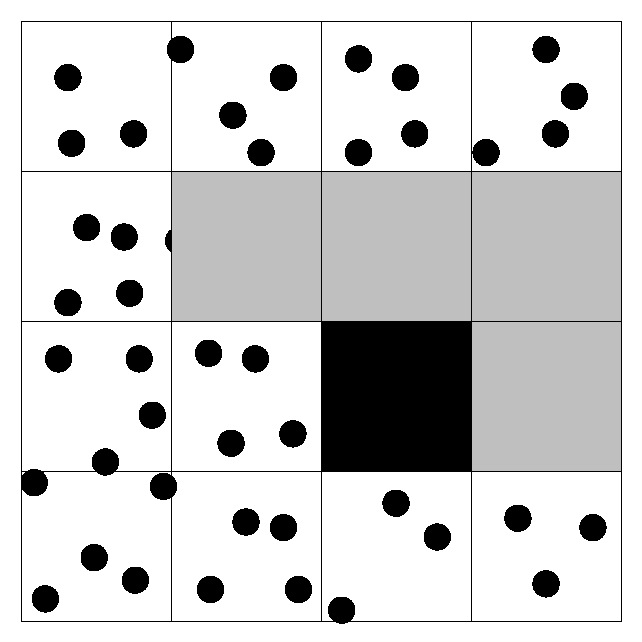
\epsfig{file=NumTech/bufzone.ps,height=7.5cm,width=7.5cm}
    \setlength{\unitlength}{0.00083333in}
%
\begingroup\makeatletter\ifx\SetFigFont\undefined
% extract first six characters in \fmtname
\def\x#1#2#3#4#5#6#7\relax{\def\x{#1#2#3#4#5#6}}%
\expandafter\x\fmtname xxxxxx\relax \def\y{splain}%
\ifx\x\y   % LaTeX or SliTeX?
\gdef\SetFigFont#1#2#3{%
  \ifnum #1<17\tiny\else \ifnum #1<20\small\else
  \ifnum #1<24\normalsize\else \ifnum #1<29\large\else
  \ifnum #1<34\Large\else \ifnum #1<41\LARGE\else
     \huge\fi\fi\fi\fi\fi\fi
  \csname #3\endcsname}%
\else
\gdef\SetFigFont#1#2#3{\begingroup
  \count@#1\relax \ifnum 25<\count@\count@25\fi
  \def\x{\endgroup\@setsize\SetFigFont{#2pt}}%
  \expandafter\x
    \csname \romannumeral\the\count@ pt\expandafter\endcsname
    \csname @\romannumeral\the\count@ pt\endcsname
  \csname #3\endcsname}%
\fi
\fi\endgroup
{\renewcommand{\dashlinestretch}{30}
\begin{picture}(4824,4839)(0,-10)
\path(12,4812)(4812,4812)(4812,3612)
	(12,3612)(12,4812)
\path(12,3612)(4812,3612)(4812,2412)
	(12,2412)(12,3612)
\path(12,2412)(4812,2412)(4812,1212)
	(12,1212)(12,2412)
\path(12,1212)(4812,1212)(4812,12)
	(12,12)(12,1212)
\put(612,4137){\makebox(0,0)[lb]{\smash{{{\SetFigFont{12}{14.4}{rm}Domain (processor) no. 1}}}}}
\put(612,2937){\makebox(0,0)[lb]{\smash{{{\SetFigFont{12}{14.4}{rm}Domain (processor) no. 2}}}}}
\put(687,1812){\makebox(0,0)[lb]{\smash{{{\SetFigFont{12}{14.4}{rm}Domain (processor) no. 3}}}}}
\put(612,612){\makebox(0,0)[lb]{\smash{{{\SetFigFont{12}{14.4}{rm}Domain (processor) no. 4}}}}}
\end{picture}
}

  \end{center}
  \caption[The cell-list method]{The simulation is partitioned into a number of
  squares. The particles in the four shaded squares may interact with the
  ones in black square.\label{fig:BuffZone}}
\end{figure}

The optimisation strategy discussed above can be expressed as
algorithm \ref{prg:OptForceCalc}. 

\begin{algorithm}
  \caption[Optimerised force calculation]{Optimerised force calculation}
  \label{prg:OptForceCalc}
  \begin{algorithmic}
    \FOR[$M$ is the number of time steps]{$p=1$ to $M$}
    \IF{$\mod(p, N_{\smbox{update}})=1$}
      \STATE \texttt{PutInBox}($\vec{r}_k$, $r_b$, $H$, $L$)
      \STATE \texttt{MakeList}($\vec{r}_k$, $r_b$, $H$, $L$, $\{i, j\}$)
    \ENDIF
    \STATE \texttt{CalcForce}($\vec{r}_k$, $\vec{F}_k$, $\{i, j\}$)
    \STATE \texttt{Integrate}($\vec{r}_k$, $\vec{v}_k$, $\vec{F}_k$)
    \ENDFOR
  \end{algorithmic}
\end{algorithm}

The procedure \texttt{PutInBox} sorts the particles into boxes
according to their positions. The algorithm is given by algorithm
\ref{prg:PutInBox}. The function $\lceil x\rceil$ returns the
largest integer $i$, that fulfills $i\le x$, where $x$ is a real
number. 

\begin{algorithm}
  \caption[\texttt{PutInBox}: Sort Particles]{\texttt{PutInBox}: Sort particles}
  \label{prg:PutInBox}
  \begin{algorithmic}
    \REQUIRE $\vec{r}_k$, $r_b$, $L$
    \FOR[$C$ is the number of cells in each direction]{$i=1$ to $C^2$}
      \STATE $H_i \leftarrow 0$ \COMMENT{Head of list for each cell}
    \ENDFOR
    \FOR{$i=1$ to $N$}
      \STATE $j \leftarrow 1+\lceil{x_i/r_b}\rceil\times
             C+\lceil{y_i/r_b}\rceil\times C^2$
             \COMMENT{$\vec{r}_i = (x_i, y_i)$}
      \STATE $L_i \leftarrow H_j$ \COMMENT{$L$ is a collection of
        linked-list of particles}
      \STATE $H_j \leftarrow i$
    \ENDFOR
  \end{algorithmic}
\end{algorithm}

The procedure \texttt{MakeList} makes a list, $\{i, j\}$, with $N_p$
elements which is a list of potentially interacting pairs of
particles. The algorithm is given as algorithm \ref{prg:MakeList}. For
simplicity, we have in algorithm \ref{prg:MakeList} neglected the loop
over the neighbouring boxes.

\begin{algorithm}
  \caption[\texttt{MakeList}: Make a list]{\texttt{MakeList}: Make a list of potentially interacting
    pairs} 
  \label{prg:MakeList}
  \begin{algorithmic}
    \REQUIRE $\vec{r}_k$, $r_b$, $H$, $L$, $N_p$, $\{i, j\}$
    \STATE $N_p \leftarrow 0$ \COMMENT{$N_p$ is the number of pairs}
    \FOR{$k=1$ to $C^2$}
      \STATE $i \leftarrow H_k$
      \WHILE{$i \ne 0$}
        \STATE $j \leftarrow H_i$
        \WHILE{$j \ne 0$}
          \IF{$\|\vec{r}_i-\vec{r}_j\|\le r_b$}
            \STATE $N_p \leftarrow N_p+1$ \COMMENT{A new pair}
            \STATE $\{i, j\}_{N_p} \leftarrow (i, j)$
          \ENDIF
          \STATE $j \leftarrow L_j$
        \ENDWHILE
      \ENDWHILE
      \STATE $i \leftarrow L_i$
    \ENDFOR
  \end{algorithmic}
\end{algorithm}

Finally, the force calculation procedure, \texttt{CalcForce}, can be
redesigned so that it takes advantage of the list of potentially interacting
pairs. The algorithm is shown as algorithm
\ref{prg:CalcForceCore}. The function \texttt{Force} calculates the
force between two particles at a given distance.

\begin{algorithm}
  \caption[\texttt{CalcForce}: force calculation]{\texttt{CalcForce}: the core of the force calculation}
  \label{prg:CalcForceCore}
  \begin{algorithmic}
    \REQUIRE $\vec{r}_k$, $\vec{F}_k$, $N_p$, $\{i, j\}$
    \FOR[Reset forces]{$m=1$ to $N$}
      \STATE $\vec{F}_i \leftarrow \vec{0}$
    \ENDFOR
    \FOR[Loop over all pairs]{$m=1$ to $N_p$}
      \STATE $(i, j) \leftarrow \{i, j\}_m$
      \STATE $\Delta\vec{r} \leftarrow \vec{r}_i-\vec{r}_j$
      \IF{$\|\Delta\vec{r}\| < r_c$}
        \STATE $\vec{f} \leftarrow$ \texttt{Force}($\Delta\vec{r}$)
        \STATE $\vec{F}_i \leftarrow \vec{F}_i+\vec{f}$
        \STATE $\vec{F}_j \leftarrow \vec{F}_j-\vec{f}$
      \ENDIF
    \ENDFOR
  \end{algorithmic}
\end{algorithm}

Figure \ref{fig:ExecTime} shows the execution time as function of the
number of particles for an MD program written by the author. We see
that the execution time grows almost linearly but this might come from the
fact that the data can easily be contained in the second-level cache.


\begin{figure}
  % GNUPLOT: LaTeX picture
\setlength{\unitlength}{0.240900pt}
\ifx\plotpoint\undefined\newsavebox{\plotpoint}\fi
\sbox{\plotpoint}{\rule[-0.200pt]{0.400pt}{0.400pt}}%
\begin{picture}(1500,900)(0,0)
\font\gnuplot=cmr10 at 10pt
\gnuplot
\sbox{\plotpoint}{\rule[-0.200pt]{0.400pt}{0.400pt}}%
\put(201.0,163.0){\rule[-0.200pt]{4.818pt}{0.400pt}}
\put(181,163){\makebox(0,0)[r]{0}}
\put(1460.0,163.0){\rule[-0.200pt]{4.818pt}{0.400pt}}
\put(201.0,250.0){\rule[-0.200pt]{4.818pt}{0.400pt}}
\put(181,250){\makebox(0,0)[r]{200}}
\put(1460.0,250.0){\rule[-0.200pt]{4.818pt}{0.400pt}}
\put(201.0,337.0){\rule[-0.200pt]{4.818pt}{0.400pt}}
\put(181,337){\makebox(0,0)[r]{400}}
\put(1460.0,337.0){\rule[-0.200pt]{4.818pt}{0.400pt}}
\put(201.0,424.0){\rule[-0.200pt]{4.818pt}{0.400pt}}
\put(181,424){\makebox(0,0)[r]{600}}
\put(1460.0,424.0){\rule[-0.200pt]{4.818pt}{0.400pt}}
\put(201.0,511.0){\rule[-0.200pt]{4.818pt}{0.400pt}}
\put(181,511){\makebox(0,0)[r]{800}}
\put(1460.0,511.0){\rule[-0.200pt]{4.818pt}{0.400pt}}
\put(201.0,598.0){\rule[-0.200pt]{4.818pt}{0.400pt}}
\put(181,598){\makebox(0,0)[r]{1000}}
\put(1460.0,598.0){\rule[-0.200pt]{4.818pt}{0.400pt}}
\put(201.0,685.0){\rule[-0.200pt]{4.818pt}{0.400pt}}
\put(181,685){\makebox(0,0)[r]{1200}}
\put(1460.0,685.0){\rule[-0.200pt]{4.818pt}{0.400pt}}
\put(201.0,772.0){\rule[-0.200pt]{4.818pt}{0.400pt}}
\put(181,772){\makebox(0,0)[r]{1400}}
\put(1460.0,772.0){\rule[-0.200pt]{4.818pt}{0.400pt}}
\put(201.0,859.0){\rule[-0.200pt]{4.818pt}{0.400pt}}
\put(181,859){\makebox(0,0)[r]{1600}}
\put(1460.0,859.0){\rule[-0.200pt]{4.818pt}{0.400pt}}
\put(201.0,163.0){\rule[-0.200pt]{0.400pt}{4.818pt}}
\put(201,122){\makebox(0,0){0}}
\put(201.0,839.0){\rule[-0.200pt]{0.400pt}{4.818pt}}
\put(361.0,163.0){\rule[-0.200pt]{0.400pt}{4.818pt}}
\put(361,122){\makebox(0,0){1000}}
\put(361.0,839.0){\rule[-0.200pt]{0.400pt}{4.818pt}}
\put(521.0,163.0){\rule[-0.200pt]{0.400pt}{4.818pt}}
\put(521,122){\makebox(0,0){2000}}
\put(521.0,839.0){\rule[-0.200pt]{0.400pt}{4.818pt}}
\put(681.0,163.0){\rule[-0.200pt]{0.400pt}{4.818pt}}
\put(681,122){\makebox(0,0){3000}}
\put(681.0,839.0){\rule[-0.200pt]{0.400pt}{4.818pt}}
\put(840.0,163.0){\rule[-0.200pt]{0.400pt}{4.818pt}}
\put(840,122){\makebox(0,0){4000}}
\put(840.0,839.0){\rule[-0.200pt]{0.400pt}{4.818pt}}
\put(1000.0,163.0){\rule[-0.200pt]{0.400pt}{4.818pt}}
\put(1000,122){\makebox(0,0){5000}}
\put(1000.0,839.0){\rule[-0.200pt]{0.400pt}{4.818pt}}
\put(1160.0,163.0){\rule[-0.200pt]{0.400pt}{4.818pt}}
\put(1160,122){\makebox(0,0){6000}}
\put(1160.0,839.0){\rule[-0.200pt]{0.400pt}{4.818pt}}
\put(1320.0,163.0){\rule[-0.200pt]{0.400pt}{4.818pt}}
\put(1320,122){\makebox(0,0){7000}}
\put(1320.0,839.0){\rule[-0.200pt]{0.400pt}{4.818pt}}
\put(1480.0,163.0){\rule[-0.200pt]{0.400pt}{4.818pt}}
\put(1480,122){\makebox(0,0){8000}}
\put(1480.0,839.0){\rule[-0.200pt]{0.400pt}{4.818pt}}
\put(201.0,163.0){\rule[-0.200pt]{308.111pt}{0.400pt}}
\put(1480.0,163.0){\rule[-0.200pt]{0.400pt}{167.666pt}}
\put(201.0,859.0){\rule[-0.200pt]{308.111pt}{0.400pt}}
\put(41,511){\makebox(0,0){\begin{rotate}{90}Execution time\end{rotate}}}
\put(840,61){\makebox(0,0){Number of particles}}
\put(201.0,163.0){\rule[-0.200pt]{0.400pt}{167.666pt}}
\put(242,187){\usebox{\plotpoint}}
\multiput(242.00,187.58)(1.069,0.495){31}{\rule{0.947pt}{0.119pt}}
\multiput(242.00,186.17)(34.034,17.000){2}{\rule{0.474pt}{0.400pt}}
\multiput(278.00,204.58)(0.928,0.498){91}{\rule{0.840pt}{0.120pt}}
\multiput(278.00,203.17)(85.256,47.000){2}{\rule{0.420pt}{0.400pt}}
\multiput(365.00,251.58)(1.076,0.499){133}{\rule{0.959pt}{0.120pt}}
\multiput(365.00,250.17)(144.010,68.000){2}{\rule{0.479pt}{0.400pt}}
\multiput(511.00,319.58)(0.994,0.499){265}{\rule{0.894pt}{0.120pt}}
\multiput(511.00,318.17)(264.144,134.000){2}{\rule{0.447pt}{0.400pt}}
\multiput(777.00,453.58)(0.900,0.498){85}{\rule{0.818pt}{0.120pt}}
\multiput(777.00,452.17)(77.302,44.000){2}{\rule{0.409pt}{0.400pt}}
\multiput(856.00,497.58)(0.985,0.500){589}{\rule{0.888pt}{0.120pt}}
\multiput(856.00,496.17)(581.157,296.000){2}{\rule{0.444pt}{0.400pt}}
\put(242,187){\raisebox{-.8pt}{\makebox(0,0){$\Diamond$}}}
\put(278,204){\raisebox{-.8pt}{\makebox(0,0){$\Diamond$}}}
\put(365,251){\raisebox{-.8pt}{\makebox(0,0){$\Diamond$}}}
\put(511,319){\raisebox{-.8pt}{\makebox(0,0){$\Diamond$}}}
\put(777,453){\raisebox{-.8pt}{\makebox(0,0){$\Diamond$}}}
\put(856,497){\raisebox{-.8pt}{\makebox(0,0){$\Diamond$}}}
\put(1439,793){\raisebox{-.8pt}{\makebox(0,0){$\Diamond$}}}
\end{picture}

  \caption[Execution time]{The execution time (in seconds) versus the number of
    particles. The density is $0.8\sigma^2$, and the temperature is $2\epsilon/k_B$.
    The execution time is the mean of 5 runs. The test was performed on an
    IBM RS/6000 Model 390 running AIX version 4.0. The
    compilation was performed using the \texttt{xlf}
    compiler.\label{fig:ExecTime}}
\end{figure}



\section{Simulating chemical reactions}
\label{sect:SimulChemReact}
One of the main interests in the work behind the present thesis is
chemical reactions. Traditionally, chemical reactions have not been
simulated by Molecular Dynamics, but a number of papers exist, see \eg
Diebner \etal \cite{Diebner95}, Heinrichs \etal \cite{Heinrichs83}, and
Ortoleva \etal \cite{Ortoleva76}. The emphasis in these papers has been
on the chemical reactions and their properties. The work presented
here is of another nature - we wish to investigate the interplay
between phase transitions and oscillating chemical reactions.

In Nature two different types of reactions exist: uni- and
bimolecular reactions. Unimolecular reactions involve one molecule
only. A typical reaction of this type is the relaxation of an excited
molecule which might dissociate it. Two molecules are involved in the
bimolecular reactions - a simple picture may be that two molecules collide
and something (the reaction) happens.

We have chosen two very simple strategies in order to simulate uni-
and bimolecular reactions. The unimolecular reaction ($A\rightarrow
P$) is a change in the label or colour of the particle. We modify the
colour with a given probability $P_r$. The algorithm is shown below.

\begin{algorithm}
  \caption[Performs the reaction $A\rightarrow P$]{Performs the reaction $A\rightarrow P$} 
  \label{prg:uni}  
  \begin{algorithmic}
    \FOR{$i=1$ to $N$}
      \STATE $p \leftarrow$ \texttt{RandUnit} 
        \COMMENT{Returns a uniformly distributed random number}
      \IF[$P_r$ is the reaction probability]{$p \le P_r$}
        \STATE Alter $i$'s label from $A$ to $P$
      \ENDIF
    \ENDFOR
  \end{algorithmic}
\end{algorithm}

A bimolecular reaction involves two
molecules. The general reaction is $A + B \rightarrow P + Q$. The
naive idea is to let the reaction occur when $A$ and $B$ collide, but
since most of the work presented here is from studies of Lennard-Jones
particles, collisions are not a well-defined term. We \textit{define}
a collision to be the event where two particles $i$ and $j$ are close
\ie the distance is less than a given number $R_{\smbox{reac}}$. Moreover,
we let the reaction happen with a given probability $P_r$ only. The
algorithm shown below uses the list of potentially interacting pairs
coming from algorithm \ref{prg:OptForceCalc} since we know that these
particles will also be the potentially reacting particles.

\begin{algorithm}
  \caption[Performs the reaction $A+B\rightarrow P+Q$]{Performs the reaction $A+B\rightarrow P+Q$}
  \label{prg:bi}
  \begin{algorithmic}
    \REQUIRE $\{i, j\}_k$
    \FOR{$k=1$ to $N_p$}
      \STATE $(i, j) \leftarrow \{i, j\}_k$
      \STATE $\Delta r \leftarrow \|\vec{r}_i-\vec{r}_j\|$
      \IF{$\Delta r \le R_{\smbox{reac}}$}
        \STATE $p \leftarrow$ \texttt{RandUnit}
        \IF{$p \le P_r$}
          \STATE Modify the labels of particles $i$ and $j$
        \ENDIF
      \ENDIF
    \ENDFOR
  \end{algorithmic}
\end{algorithm}

The parameters, $R_{\smbox{reac}}$ and $P_r$, introduced above define
the reaction rate. The rate of a reaction is, in traditional chemical
kinetics, measured by the rate constant; see section
\ref{sect:MeasureRate} for details about the measurement of the rate
constants. One of the most successful theories of reaction rate is the
collision theory, see \eg Pilling \etal \cite{Pilling95}. The idea
behind the collision theory of reaction rates is that two reactants,
$X$ and $Y$, collide and form an encounter pair, $C$. The encounter
pair will either form the reactants again or a product, $P$. In
terms of reactions, the reaction $X+Y \rightarrow P$ is the overall
reaction of the three subreactions $X+Y \rightleftarrows C \rightarrow
P$. Let $\vec{r}_X$ and $\vec{r}_Y$ denote the centre of mass of the two
reactant molecules, respectively. A collision is then the event that
$\|\vec{r}_X - \vec{r}_Y\| \le R_{\smbox{reac}}$ \ie the distance
between the reactants is less than some predefined value,
$R_{\smbox{reac}}$. When the reactants are closer to each other that 
$R_{\smbox{reac}}$, they form the encounter pair $C$. The encounter
pair will - as already mentioned - form either the products or the
reactants. The probability of forming the product is $P_r$, and the
probability of a non-reactive collision (forming the reactants) is
$1-P_r$.


\section{Parallelisation}
\label{sect:Parallel}
The modern supercomputer is a parallel computer, and the use of these
computers becomes more and more popular. Two different approaches to
the parallel computer exist; distributed and shared 
memory computers, see \eg Tanenbaum \cite{Tanenbaum90}. The
characteristics are: 

\begin{description}
\item[Shared memory] A number of processors (cpus) are using
  the same pool of storage (or memory) and system resources \eg I/O
  units. A computer of this type is PowerChallenger (Silicon
  Graphics Inc.). If processor $i$ needs a piece of data, it can read it at
  any time in the storage independent of what processor $j$ is doing. 
\item[Distributed memory] Each processor has a private storage and
  often private I/O units. When processor $i$ needs data stored in
  processor $j$'s storage, a communication link is established. The 
  communication is slow compared to direct access to the storage, and
  communication must be minimised. This type of parallel computer can
  be built by a number of connected workstations. Typical high-end
  solutions are RS/6000 SP (International Business Machines) and T3E
  (Cray Research). 
\end{description}

We have had access to an RS/6000 SP computer situated at
Uni$\bullet$C\footnote{The Danish Computing Centre for Research and Education.
The home page of the computer is \texttt{http://www.sp2.uni-c.dk}.} and
in the following we will describe our parallelisation strategy.

Systems simulated by Molecular Dynamics are spatial by their nature. It
is ``obvious'' to let a number of processors simulate a region of the
simulation cell each. This is the idea behind the parallelisation strategy
called domain decomposition, see \eg Brown \etal
\cite{Brown93}. Figure \ref{fig:DomainDecomp} shows a simulation cell
which has been divided into four domains. The particles which are
situated in a given domain, are simulated by a given processor \ie
each processor simulates a region of the simulation cell. When a
particle moves out of the domain of one processor and into the domain
of the neighbouring processor, its position and velocity is sent to
the new processor. 

\begin{figure}
  \begin{center}
    \input{NumTech/multicpu.eepic}
  \end{center}
  \caption[Domain decomposition]{The simulation is divided into a
  number of domains - one for each processor. The subcell structure is
  also shown.\label{fig:DomainDecomp}} 
\end{figure}

In section \ref{sect:OptForceCalc} we discussed an optimisation
strategy, namely dividing the simulation cell into a number of
boxes. The boxes are much smaller than the simulation cell, and
even with the domain decomposition many boxes will reside on each
processor. Of course we can still use the box idea, and
even better, we can use it for optimising the domain decomposition. At
each time step in principle each processor needs to know the positions
of all particles in order to calculate the forces. But the idea behind
the optimisation trick in section \ref{sect:OptForceCalc} is that
particles far from each other will not interact. Therefore
only particles which are located in the subcells close to the
boundaries of a processor's domain will interact with the particles
situated on the neighbouring processor. Then, only the positions of
these particles have to be communicated. 

Figure \ref{fig:ParallelSpeed} shows the execution times for a
Molecular Dynamics program which has been parallelised by the domain
decomposition. We do not see a linear speed-up but up to 8 processors
we only ``pay'' 25 percent of the execution time for parallelisation.

\begin{figure}
  \begin{center}
    % GNUPLOT: LaTeX picture
\setlength{\unitlength}{0.240900pt}
\ifx\plotpoint\undefined\newsavebox{\plotpoint}\fi
\sbox{\plotpoint}{\rule[-0.200pt]{0.400pt}{0.400pt}}%
\begin{picture}(1500,900)(0,0)
\font\gnuplot=cmr10 at 10pt
\gnuplot
\sbox{\plotpoint}{\rule[-0.200pt]{0.400pt}{0.400pt}}%
\put(161.0,163.0){\rule[-0.200pt]{4.818pt}{0.400pt}}
\put(141,163){\makebox(0,0)[r]{0}}
\put(1460.0,163.0){\rule[-0.200pt]{4.818pt}{0.400pt}}
\put(161.0,221.0){\rule[-0.200pt]{2.409pt}{0.400pt}}
\put(1470.0,221.0){\rule[-0.200pt]{2.409pt}{0.400pt}}
\put(161.0,279.0){\rule[-0.200pt]{4.818pt}{0.400pt}}
\put(141,279){\makebox(0,0)[r]{2}}
\put(1460.0,279.0){\rule[-0.200pt]{4.818pt}{0.400pt}}
\put(161.0,337.0){\rule[-0.200pt]{2.409pt}{0.400pt}}
\put(1470.0,337.0){\rule[-0.200pt]{2.409pt}{0.400pt}}
\put(161.0,395.0){\rule[-0.200pt]{4.818pt}{0.400pt}}
\put(141,395){\makebox(0,0)[r]{4}}
\put(1460.0,395.0){\rule[-0.200pt]{4.818pt}{0.400pt}}
\put(161.0,453.0){\rule[-0.200pt]{2.409pt}{0.400pt}}
\put(1470.0,453.0){\rule[-0.200pt]{2.409pt}{0.400pt}}
\put(161.0,511.0){\rule[-0.200pt]{4.818pt}{0.400pt}}
\put(141,511){\makebox(0,0)[r]{6}}
\put(1460.0,511.0){\rule[-0.200pt]{4.818pt}{0.400pt}}
\put(161.0,569.0){\rule[-0.200pt]{2.409pt}{0.400pt}}
\put(1470.0,569.0){\rule[-0.200pt]{2.409pt}{0.400pt}}
\put(161.0,627.0){\rule[-0.200pt]{4.818pt}{0.400pt}}
\put(141,627){\makebox(0,0)[r]{8}}
\put(1460.0,627.0){\rule[-0.200pt]{4.818pt}{0.400pt}}
\put(161.0,685.0){\rule[-0.200pt]{2.409pt}{0.400pt}}
\put(1470.0,685.0){\rule[-0.200pt]{2.409pt}{0.400pt}}
\put(161.0,743.0){\rule[-0.200pt]{4.818pt}{0.400pt}}
\put(141,743){\makebox(0,0)[r]{10}}
\put(1460.0,743.0){\rule[-0.200pt]{4.818pt}{0.400pt}}
\put(161.0,801.0){\rule[-0.200pt]{2.409pt}{0.400pt}}
\put(1470.0,801.0){\rule[-0.200pt]{2.409pt}{0.400pt}}
\put(161.0,859.0){\rule[-0.200pt]{4.818pt}{0.400pt}}
\put(141,859){\makebox(0,0)[r]{12}}
\put(1460.0,859.0){\rule[-0.200pt]{4.818pt}{0.400pt}}
\put(161.0,163.0){\rule[-0.200pt]{0.400pt}{4.818pt}}
\put(161,122){\makebox(0,0){0}}
\put(161.0,839.0){\rule[-0.200pt]{0.400pt}{4.818pt}}
\put(271.0,163.0){\rule[-0.200pt]{0.400pt}{2.409pt}}
\put(271.0,849.0){\rule[-0.200pt]{0.400pt}{2.409pt}}
\put(381.0,163.0){\rule[-0.200pt]{0.400pt}{4.818pt}}
\put(381,122){\makebox(0,0){2}}
\put(381.0,839.0){\rule[-0.200pt]{0.400pt}{4.818pt}}
\put(491.0,163.0){\rule[-0.200pt]{0.400pt}{2.409pt}}
\put(491.0,849.0){\rule[-0.200pt]{0.400pt}{2.409pt}}
\put(601.0,163.0){\rule[-0.200pt]{0.400pt}{4.818pt}}
\put(601,122){\makebox(0,0){4}}
\put(601.0,839.0){\rule[-0.200pt]{0.400pt}{4.818pt}}
\put(711.0,163.0){\rule[-0.200pt]{0.400pt}{2.409pt}}
\put(711.0,849.0){\rule[-0.200pt]{0.400pt}{2.409pt}}
\put(821.0,163.0){\rule[-0.200pt]{0.400pt}{4.818pt}}
\put(821,122){\makebox(0,0){6}}
\put(821.0,839.0){\rule[-0.200pt]{0.400pt}{4.818pt}}
\put(930.0,163.0){\rule[-0.200pt]{0.400pt}{2.409pt}}
\put(930.0,849.0){\rule[-0.200pt]{0.400pt}{2.409pt}}
\put(1040.0,163.0){\rule[-0.200pt]{0.400pt}{4.818pt}}
\put(1040,122){\makebox(0,0){8}}
\put(1040.0,839.0){\rule[-0.200pt]{0.400pt}{4.818pt}}
\put(1150.0,163.0){\rule[-0.200pt]{0.400pt}{2.409pt}}
\put(1150.0,849.0){\rule[-0.200pt]{0.400pt}{2.409pt}}
\put(1260.0,163.0){\rule[-0.200pt]{0.400pt}{4.818pt}}
\put(1260,122){\makebox(0,0){10}}
\put(1260.0,839.0){\rule[-0.200pt]{0.400pt}{4.818pt}}
\put(1370.0,163.0){\rule[-0.200pt]{0.400pt}{2.409pt}}
\put(1370.0,849.0){\rule[-0.200pt]{0.400pt}{2.409pt}}
\put(1480.0,163.0){\rule[-0.200pt]{0.400pt}{4.818pt}}
\put(1480,122){\makebox(0,0){12}}
\put(1480.0,839.0){\rule[-0.200pt]{0.400pt}{4.818pt}}
\put(161.0,163.0){\rule[-0.200pt]{317.747pt}{0.400pt}}
\put(1480.0,163.0){\rule[-0.200pt]{0.400pt}{167.666pt}}
\put(161.0,859.0){\rule[-0.200pt]{317.747pt}{0.400pt}}
\put(41,511){\makebox(0,0){\begin{rotate}{90}Speed-up\end{rotate}}}
\put(820,61){\makebox(0,0){No. processors}}
\put(161.0,163.0){\rule[-0.200pt]{0.400pt}{167.666pt}}
\put(161,163){\usebox{\plotpoint}}
\multiput(161.00,163.59)(0.950,0.485){11}{\rule{0.843pt}{0.117pt}}
\multiput(161.00,162.17)(11.251,7.000){2}{\rule{0.421pt}{0.400pt}}
\multiput(174.00,170.59)(1.026,0.485){11}{\rule{0.900pt}{0.117pt}}
\multiput(174.00,169.17)(12.132,7.000){2}{\rule{0.450pt}{0.400pt}}
\multiput(188.00,177.59)(0.950,0.485){11}{\rule{0.843pt}{0.117pt}}
\multiput(188.00,176.17)(11.251,7.000){2}{\rule{0.421pt}{0.400pt}}
\multiput(201.00,184.59)(0.950,0.485){11}{\rule{0.843pt}{0.117pt}}
\multiput(201.00,183.17)(11.251,7.000){2}{\rule{0.421pt}{0.400pt}}
\multiput(214.00,191.59)(1.026,0.485){11}{\rule{0.900pt}{0.117pt}}
\multiput(214.00,190.17)(12.132,7.000){2}{\rule{0.450pt}{0.400pt}}
\multiput(228.00,198.59)(0.950,0.485){11}{\rule{0.843pt}{0.117pt}}
\multiput(228.00,197.17)(11.251,7.000){2}{\rule{0.421pt}{0.400pt}}
\multiput(241.00,205.59)(0.950,0.485){11}{\rule{0.843pt}{0.117pt}}
\multiput(241.00,204.17)(11.251,7.000){2}{\rule{0.421pt}{0.400pt}}
\multiput(254.00,212.59)(1.026,0.485){11}{\rule{0.900pt}{0.117pt}}
\multiput(254.00,211.17)(12.132,7.000){2}{\rule{0.450pt}{0.400pt}}
\multiput(268.00,219.59)(0.950,0.485){11}{\rule{0.843pt}{0.117pt}}
\multiput(268.00,218.17)(11.251,7.000){2}{\rule{0.421pt}{0.400pt}}
\multiput(281.00,226.59)(0.950,0.485){11}{\rule{0.843pt}{0.117pt}}
\multiput(281.00,225.17)(11.251,7.000){2}{\rule{0.421pt}{0.400pt}}
\multiput(294.00,233.59)(1.026,0.485){11}{\rule{0.900pt}{0.117pt}}
\multiput(294.00,232.17)(12.132,7.000){2}{\rule{0.450pt}{0.400pt}}
\multiput(308.00,240.59)(0.950,0.485){11}{\rule{0.843pt}{0.117pt}}
\multiput(308.00,239.17)(11.251,7.000){2}{\rule{0.421pt}{0.400pt}}
\multiput(321.00,247.59)(0.950,0.485){11}{\rule{0.843pt}{0.117pt}}
\multiput(321.00,246.17)(11.251,7.000){2}{\rule{0.421pt}{0.400pt}}
\multiput(334.00,254.59)(1.026,0.485){11}{\rule{0.900pt}{0.117pt}}
\multiput(334.00,253.17)(12.132,7.000){2}{\rule{0.450pt}{0.400pt}}
\multiput(348.00,261.59)(0.950,0.485){11}{\rule{0.843pt}{0.117pt}}
\multiput(348.00,260.17)(11.251,7.000){2}{\rule{0.421pt}{0.400pt}}
\multiput(361.00,268.59)(0.950,0.485){11}{\rule{0.843pt}{0.117pt}}
\multiput(361.00,267.17)(11.251,7.000){2}{\rule{0.421pt}{0.400pt}}
\multiput(374.00,275.59)(0.824,0.488){13}{\rule{0.750pt}{0.117pt}}
\multiput(374.00,274.17)(11.443,8.000){2}{\rule{0.375pt}{0.400pt}}
\multiput(387.00,283.59)(1.026,0.485){11}{\rule{0.900pt}{0.117pt}}
\multiput(387.00,282.17)(12.132,7.000){2}{\rule{0.450pt}{0.400pt}}
\multiput(401.00,290.59)(0.950,0.485){11}{\rule{0.843pt}{0.117pt}}
\multiput(401.00,289.17)(11.251,7.000){2}{\rule{0.421pt}{0.400pt}}
\multiput(414.00,297.59)(0.950,0.485){11}{\rule{0.843pt}{0.117pt}}
\multiput(414.00,296.17)(11.251,7.000){2}{\rule{0.421pt}{0.400pt}}
\multiput(427.00,304.59)(1.026,0.485){11}{\rule{0.900pt}{0.117pt}}
\multiput(427.00,303.17)(12.132,7.000){2}{\rule{0.450pt}{0.400pt}}
\multiput(441.00,311.59)(0.950,0.485){11}{\rule{0.843pt}{0.117pt}}
\multiput(441.00,310.17)(11.251,7.000){2}{\rule{0.421pt}{0.400pt}}
\multiput(454.00,318.59)(0.950,0.485){11}{\rule{0.843pt}{0.117pt}}
\multiput(454.00,317.17)(11.251,7.000){2}{\rule{0.421pt}{0.400pt}}
\multiput(467.00,325.59)(1.026,0.485){11}{\rule{0.900pt}{0.117pt}}
\multiput(467.00,324.17)(12.132,7.000){2}{\rule{0.450pt}{0.400pt}}
\multiput(481.00,332.59)(0.950,0.485){11}{\rule{0.843pt}{0.117pt}}
\multiput(481.00,331.17)(11.251,7.000){2}{\rule{0.421pt}{0.400pt}}
\multiput(494.00,339.59)(0.950,0.485){11}{\rule{0.843pt}{0.117pt}}
\multiput(494.00,338.17)(11.251,7.000){2}{\rule{0.421pt}{0.400pt}}
\multiput(507.00,346.59)(1.026,0.485){11}{\rule{0.900pt}{0.117pt}}
\multiput(507.00,345.17)(12.132,7.000){2}{\rule{0.450pt}{0.400pt}}
\multiput(521.00,353.59)(0.950,0.485){11}{\rule{0.843pt}{0.117pt}}
\multiput(521.00,352.17)(11.251,7.000){2}{\rule{0.421pt}{0.400pt}}
\multiput(534.00,360.59)(0.950,0.485){11}{\rule{0.843pt}{0.117pt}}
\multiput(534.00,359.17)(11.251,7.000){2}{\rule{0.421pt}{0.400pt}}
\multiput(547.00,367.59)(1.026,0.485){11}{\rule{0.900pt}{0.117pt}}
\multiput(547.00,366.17)(12.132,7.000){2}{\rule{0.450pt}{0.400pt}}
\multiput(561.00,374.59)(0.950,0.485){11}{\rule{0.843pt}{0.117pt}}
\multiput(561.00,373.17)(11.251,7.000){2}{\rule{0.421pt}{0.400pt}}
\multiput(574.00,381.59)(0.950,0.485){11}{\rule{0.843pt}{0.117pt}}
\multiput(574.00,380.17)(11.251,7.000){2}{\rule{0.421pt}{0.400pt}}
\multiput(587.00,388.59)(1.026,0.485){11}{\rule{0.900pt}{0.117pt}}
\multiput(587.00,387.17)(12.132,7.000){2}{\rule{0.450pt}{0.400pt}}
\multiput(601.00,395.59)(0.950,0.485){11}{\rule{0.843pt}{0.117pt}}
\multiput(601.00,394.17)(11.251,7.000){2}{\rule{0.421pt}{0.400pt}}
\multiput(614.00,402.59)(0.950,0.485){11}{\rule{0.843pt}{0.117pt}}
\multiput(614.00,401.17)(11.251,7.000){2}{\rule{0.421pt}{0.400pt}}
\multiput(627.00,409.59)(1.026,0.485){11}{\rule{0.900pt}{0.117pt}}
\multiput(627.00,408.17)(12.132,7.000){2}{\rule{0.450pt}{0.400pt}}
\multiput(641.00,416.59)(0.950,0.485){11}{\rule{0.843pt}{0.117pt}}
\multiput(641.00,415.17)(11.251,7.000){2}{\rule{0.421pt}{0.400pt}}
\multiput(654.00,423.59)(0.950,0.485){11}{\rule{0.843pt}{0.117pt}}
\multiput(654.00,422.17)(11.251,7.000){2}{\rule{0.421pt}{0.400pt}}
\multiput(667.00,430.59)(1.026,0.485){11}{\rule{0.900pt}{0.117pt}}
\multiput(667.00,429.17)(12.132,7.000){2}{\rule{0.450pt}{0.400pt}}
\multiput(681.00,437.59)(0.950,0.485){11}{\rule{0.843pt}{0.117pt}}
\multiput(681.00,436.17)(11.251,7.000){2}{\rule{0.421pt}{0.400pt}}
\multiput(694.00,444.59)(0.950,0.485){11}{\rule{0.843pt}{0.117pt}}
\multiput(694.00,443.17)(11.251,7.000){2}{\rule{0.421pt}{0.400pt}}
\multiput(707.00,451.59)(1.026,0.485){11}{\rule{0.900pt}{0.117pt}}
\multiput(707.00,450.17)(12.132,7.000){2}{\rule{0.450pt}{0.400pt}}
\multiput(721.00,458.59)(0.950,0.485){11}{\rule{0.843pt}{0.117pt}}
\multiput(721.00,457.17)(11.251,7.000){2}{\rule{0.421pt}{0.400pt}}
\multiput(734.00,465.59)(0.950,0.485){11}{\rule{0.843pt}{0.117pt}}
\multiput(734.00,464.17)(11.251,7.000){2}{\rule{0.421pt}{0.400pt}}
\multiput(747.00,472.59)(1.026,0.485){11}{\rule{0.900pt}{0.117pt}}
\multiput(747.00,471.17)(12.132,7.000){2}{\rule{0.450pt}{0.400pt}}
\multiput(761.00,479.59)(0.950,0.485){11}{\rule{0.843pt}{0.117pt}}
\multiput(761.00,478.17)(11.251,7.000){2}{\rule{0.421pt}{0.400pt}}
\multiput(774.00,486.59)(0.950,0.485){11}{\rule{0.843pt}{0.117pt}}
\multiput(774.00,485.17)(11.251,7.000){2}{\rule{0.421pt}{0.400pt}}
\multiput(787.00,493.59)(1.026,0.485){11}{\rule{0.900pt}{0.117pt}}
\multiput(787.00,492.17)(12.132,7.000){2}{\rule{0.450pt}{0.400pt}}
\multiput(801.00,500.59)(0.950,0.485){11}{\rule{0.843pt}{0.117pt}}
\multiput(801.00,499.17)(11.251,7.000){2}{\rule{0.421pt}{0.400pt}}
\multiput(814.00,507.59)(0.824,0.488){13}{\rule{0.750pt}{0.117pt}}
\multiput(814.00,506.17)(11.443,8.000){2}{\rule{0.375pt}{0.400pt}}
\multiput(827.00,515.59)(0.950,0.485){11}{\rule{0.843pt}{0.117pt}}
\multiput(827.00,514.17)(11.251,7.000){2}{\rule{0.421pt}{0.400pt}}
\multiput(840.00,522.59)(1.026,0.485){11}{\rule{0.900pt}{0.117pt}}
\multiput(840.00,521.17)(12.132,7.000){2}{\rule{0.450pt}{0.400pt}}
\multiput(854.00,529.59)(0.950,0.485){11}{\rule{0.843pt}{0.117pt}}
\multiput(854.00,528.17)(11.251,7.000){2}{\rule{0.421pt}{0.400pt}}
\multiput(867.00,536.59)(0.950,0.485){11}{\rule{0.843pt}{0.117pt}}
\multiput(867.00,535.17)(11.251,7.000){2}{\rule{0.421pt}{0.400pt}}
\multiput(880.00,543.59)(1.026,0.485){11}{\rule{0.900pt}{0.117pt}}
\multiput(880.00,542.17)(12.132,7.000){2}{\rule{0.450pt}{0.400pt}}
\multiput(894.00,550.59)(0.950,0.485){11}{\rule{0.843pt}{0.117pt}}
\multiput(894.00,549.17)(11.251,7.000){2}{\rule{0.421pt}{0.400pt}}
\multiput(907.00,557.59)(0.950,0.485){11}{\rule{0.843pt}{0.117pt}}
\multiput(907.00,556.17)(11.251,7.000){2}{\rule{0.421pt}{0.400pt}}
\multiput(920.00,564.59)(1.026,0.485){11}{\rule{0.900pt}{0.117pt}}
\multiput(920.00,563.17)(12.132,7.000){2}{\rule{0.450pt}{0.400pt}}
\multiput(934.00,571.59)(0.950,0.485){11}{\rule{0.843pt}{0.117pt}}
\multiput(934.00,570.17)(11.251,7.000){2}{\rule{0.421pt}{0.400pt}}
\multiput(947.00,578.59)(0.950,0.485){11}{\rule{0.843pt}{0.117pt}}
\multiput(947.00,577.17)(11.251,7.000){2}{\rule{0.421pt}{0.400pt}}
\multiput(960.00,585.59)(1.026,0.485){11}{\rule{0.900pt}{0.117pt}}
\multiput(960.00,584.17)(12.132,7.000){2}{\rule{0.450pt}{0.400pt}}
\multiput(974.00,592.59)(0.950,0.485){11}{\rule{0.843pt}{0.117pt}}
\multiput(974.00,591.17)(11.251,7.000){2}{\rule{0.421pt}{0.400pt}}
\multiput(987.00,599.59)(0.950,0.485){11}{\rule{0.843pt}{0.117pt}}
\multiput(987.00,598.17)(11.251,7.000){2}{\rule{0.421pt}{0.400pt}}
\multiput(1000.00,606.59)(1.026,0.485){11}{\rule{0.900pt}{0.117pt}}
\multiput(1000.00,605.17)(12.132,7.000){2}{\rule{0.450pt}{0.400pt}}
\multiput(1014.00,613.59)(0.950,0.485){11}{\rule{0.843pt}{0.117pt}}
\multiput(1014.00,612.17)(11.251,7.000){2}{\rule{0.421pt}{0.400pt}}
\multiput(1027.00,620.59)(0.950,0.485){11}{\rule{0.843pt}{0.117pt}}
\multiput(1027.00,619.17)(11.251,7.000){2}{\rule{0.421pt}{0.400pt}}
\multiput(1040.00,627.59)(1.026,0.485){11}{\rule{0.900pt}{0.117pt}}
\multiput(1040.00,626.17)(12.132,7.000){2}{\rule{0.450pt}{0.400pt}}
\multiput(1054.00,634.59)(0.950,0.485){11}{\rule{0.843pt}{0.117pt}}
\multiput(1054.00,633.17)(11.251,7.000){2}{\rule{0.421pt}{0.400pt}}
\multiput(1067.00,641.59)(0.950,0.485){11}{\rule{0.843pt}{0.117pt}}
\multiput(1067.00,640.17)(11.251,7.000){2}{\rule{0.421pt}{0.400pt}}
\multiput(1080.00,648.59)(1.026,0.485){11}{\rule{0.900pt}{0.117pt}}
\multiput(1080.00,647.17)(12.132,7.000){2}{\rule{0.450pt}{0.400pt}}
\multiput(1094.00,655.59)(0.950,0.485){11}{\rule{0.843pt}{0.117pt}}
\multiput(1094.00,654.17)(11.251,7.000){2}{\rule{0.421pt}{0.400pt}}
\multiput(1107.00,662.59)(0.950,0.485){11}{\rule{0.843pt}{0.117pt}}
\multiput(1107.00,661.17)(11.251,7.000){2}{\rule{0.421pt}{0.400pt}}
\multiput(1120.00,669.59)(1.026,0.485){11}{\rule{0.900pt}{0.117pt}}
\multiput(1120.00,668.17)(12.132,7.000){2}{\rule{0.450pt}{0.400pt}}
\multiput(1134.00,676.59)(0.950,0.485){11}{\rule{0.843pt}{0.117pt}}
\multiput(1134.00,675.17)(11.251,7.000){2}{\rule{0.421pt}{0.400pt}}
\multiput(1147.00,683.59)(0.950,0.485){11}{\rule{0.843pt}{0.117pt}}
\multiput(1147.00,682.17)(11.251,7.000){2}{\rule{0.421pt}{0.400pt}}
\multiput(1160.00,690.59)(1.026,0.485){11}{\rule{0.900pt}{0.117pt}}
\multiput(1160.00,689.17)(12.132,7.000){2}{\rule{0.450pt}{0.400pt}}
\multiput(1174.00,697.59)(0.950,0.485){11}{\rule{0.843pt}{0.117pt}}
\multiput(1174.00,696.17)(11.251,7.000){2}{\rule{0.421pt}{0.400pt}}
\multiput(1187.00,704.59)(0.950,0.485){11}{\rule{0.843pt}{0.117pt}}
\multiput(1187.00,703.17)(11.251,7.000){2}{\rule{0.421pt}{0.400pt}}
\multiput(1200.00,711.59)(1.026,0.485){11}{\rule{0.900pt}{0.117pt}}
\multiput(1200.00,710.17)(12.132,7.000){2}{\rule{0.450pt}{0.400pt}}
\multiput(1214.00,718.59)(0.950,0.485){11}{\rule{0.843pt}{0.117pt}}
\multiput(1214.00,717.17)(11.251,7.000){2}{\rule{0.421pt}{0.400pt}}
\multiput(1227.00,725.59)(0.950,0.485){11}{\rule{0.843pt}{0.117pt}}
\multiput(1227.00,724.17)(11.251,7.000){2}{\rule{0.421pt}{0.400pt}}
\multiput(1240.00,732.59)(1.026,0.485){11}{\rule{0.900pt}{0.117pt}}
\multiput(1240.00,731.17)(12.132,7.000){2}{\rule{0.450pt}{0.400pt}}
\multiput(1254.00,739.59)(0.824,0.488){13}{\rule{0.750pt}{0.117pt}}
\multiput(1254.00,738.17)(11.443,8.000){2}{\rule{0.375pt}{0.400pt}}
\multiput(1267.00,747.59)(0.950,0.485){11}{\rule{0.843pt}{0.117pt}}
\multiput(1267.00,746.17)(11.251,7.000){2}{\rule{0.421pt}{0.400pt}}
\multiput(1280.00,754.59)(0.950,0.485){11}{\rule{0.843pt}{0.117pt}}
\multiput(1280.00,753.17)(11.251,7.000){2}{\rule{0.421pt}{0.400pt}}
\multiput(1293.00,761.59)(1.026,0.485){11}{\rule{0.900pt}{0.117pt}}
\multiput(1293.00,760.17)(12.132,7.000){2}{\rule{0.450pt}{0.400pt}}
\multiput(1307.00,768.59)(0.950,0.485){11}{\rule{0.843pt}{0.117pt}}
\multiput(1307.00,767.17)(11.251,7.000){2}{\rule{0.421pt}{0.400pt}}
\multiput(1320.00,775.59)(0.950,0.485){11}{\rule{0.843pt}{0.117pt}}
\multiput(1320.00,774.17)(11.251,7.000){2}{\rule{0.421pt}{0.400pt}}
\multiput(1333.00,782.59)(1.026,0.485){11}{\rule{0.900pt}{0.117pt}}
\multiput(1333.00,781.17)(12.132,7.000){2}{\rule{0.450pt}{0.400pt}}
\multiput(1347.00,789.59)(0.950,0.485){11}{\rule{0.843pt}{0.117pt}}
\multiput(1347.00,788.17)(11.251,7.000){2}{\rule{0.421pt}{0.400pt}}
\multiput(1360.00,796.59)(0.950,0.485){11}{\rule{0.843pt}{0.117pt}}
\multiput(1360.00,795.17)(11.251,7.000){2}{\rule{0.421pt}{0.400pt}}
\multiput(1373.00,803.59)(1.026,0.485){11}{\rule{0.900pt}{0.117pt}}
\multiput(1373.00,802.17)(12.132,7.000){2}{\rule{0.450pt}{0.400pt}}
\multiput(1387.00,810.59)(0.950,0.485){11}{\rule{0.843pt}{0.117pt}}
\multiput(1387.00,809.17)(11.251,7.000){2}{\rule{0.421pt}{0.400pt}}
\multiput(1400.00,817.59)(0.950,0.485){11}{\rule{0.843pt}{0.117pt}}
\multiput(1400.00,816.17)(11.251,7.000){2}{\rule{0.421pt}{0.400pt}}
\multiput(1413.00,824.59)(1.026,0.485){11}{\rule{0.900pt}{0.117pt}}
\multiput(1413.00,823.17)(12.132,7.000){2}{\rule{0.450pt}{0.400pt}}
\multiput(1427.00,831.59)(0.950,0.485){11}{\rule{0.843pt}{0.117pt}}
\multiput(1427.00,830.17)(11.251,7.000){2}{\rule{0.421pt}{0.400pt}}
\multiput(1440.00,838.59)(0.950,0.485){11}{\rule{0.843pt}{0.117pt}}
\multiput(1440.00,837.17)(11.251,7.000){2}{\rule{0.421pt}{0.400pt}}
\multiput(1453.00,845.59)(1.026,0.485){11}{\rule{0.900pt}{0.117pt}}
\multiput(1453.00,844.17)(12.132,7.000){2}{\rule{0.450pt}{0.400pt}}
\multiput(1467.00,852.59)(0.950,0.485){11}{\rule{0.843pt}{0.117pt}}
\multiput(1467.00,851.17)(11.251,7.000){2}{\rule{0.421pt}{0.400pt}}
\put(271,221){\usebox{\plotpoint}}
\multiput(271,221)(18.221,9.939){7}{\usebox{\plotpoint}}
\multiput(381,281)(19.149,8.008){5}{\usebox{\plotpoint}}
\multiput(491,327)(19.390,7.404){6}{\usebox{\plotpoint}}
\multiput(601,369)(19.752,6.375){11}{\usebox{\plotpoint}}
\multiput(821,440)(20.064,5.314){11}{\usebox{\plotpoint}}
\multiput(1040,498)(20.468,3.442){22}{\usebox{\plotpoint}}
\put(1480,572){\usebox{\plotpoint}}
\put(271,221){\raisebox{-.8pt}{\makebox(0,0){$\Diamond$}}}
\put(381,281){\raisebox{-.8pt}{\makebox(0,0){$\Diamond$}}}
\put(491,327){\raisebox{-.8pt}{\makebox(0,0){$\Diamond$}}}
\put(601,369){\raisebox{-.8pt}{\makebox(0,0){$\Diamond$}}}
\put(821,440){\raisebox{-.8pt}{\makebox(0,0){$\Diamond$}}}
\put(1040,498){\raisebox{-.8pt}{\makebox(0,0){$\Diamond$}}}
\put(1480,572){\raisebox{-.8pt}{\makebox(0,0){$\Diamond$}}}
\end{picture}

  \end{center}
  \caption[The speed-up of a parallel MD program]{The speed-up of a
   parallel Molecular Dynamics program. The number of Lennard-Jones
   particles is $65536$, the density is $0.8\sigma^2$ and the
   temperature is $2.0\epsilon/k_B$. The scale is relative to one processor (the serial
   program). The line with slope 1 is the linear speed-up which is the
   maximum speed-up which can be achieved.\label{fig:ParallelSpeed}}
\end{figure}


\section{Hard spheres}
\label{sect:HardSpheres}
Systems consisting of hard spheres are very different from
simulation of Lennard-Jones systems. The interaction potential is
fundamentally different because it is discontinuous \ie

\begin{equation}
  u(r) = \begin{cases}
    \infty & \text{for $r\le 2\sigma$} \\
    0      & \text{otherwise}
  \end{cases}
\end{equation}
where $\sigma$ is the radius of the particles.

As the potential indicates, the hard spheres cannot overlap. The only
interactions between the particles are through collisions, and between
collisions the particles move in straight lines (no external field is
applied). These observations show that we cannot apply the same
simulation strategy as the one for Lennard-Jones particles. 

Let us in the following discussion assume that all hard spheres have
the same radius $\sigma$, and mass $m$. Typically, we will set the mass
to unity. 

\subsection{The main loop}
\label{sect:HSnaive}
The main loop of a hard sphere simulation program is simple. Since the
only interactions are the collisions, we have to find the next
collision, update the positions and velocities and start all over
again. Algorithm \ref{prg:HSmain} shows the main loop.

\begin{algorithm}
  \caption[Hard sphere MD program]{The main loop of a hard sphere program}
  \label{prg:HSmain}
  \begin{algorithmic}
    \STATE $t \leftarrow 0$
    \WHILE{$t \leq t_{\smbox{end}}$}
      \STATE Find next collision \COMMENT{$\Delta t$ is the time until
        the next collision}
      \STATE Update positions and velocities
      \STATE Collect data
      \STATE $t \leftarrow t+\Delta t$
    \ENDWHILE
  \end{algorithmic}
\end{algorithm}


\subsection{Updating positions and velocities}
Since there is no external field, the hard spheres move in straight
lines between collisions. The positions of the particles are easily
updated; this is done by applying

\begin{equation}
\label{eq:HSeom1}
  \vec{r}_i(t+\Delta t) = \vec{r}_i(t) + \Delta t\vec{v}_i(t)
\end{equation}
for $i=1,\ldots, N$. The time difference $\Delta t$ is smaller (or
equal) to the time between two collisions. In practice we choose
$\Delta t$ to be the time until the next collision - see section
\ref{sect:Track1d}.

The velocities are only changed at collisions, and only the velocities
of the two spheres colliding are changed. It is convenient to
introduce a measurement of the inelasticity of the
collisions, which we denote $\epsilon$. The quantity $\epsilon$ is
related to the restitution coefficient $r$ as
$\epsilon=\frac{1-r}{2}$. When $\epsilon = \half$ a collision is
completely inelastic, and $\epsilon = 0$ is the completely elastic
case. The velocities are updated as

\begin{subequations}
  \begin{eqnarray}
    \vec{v}_i^{\prime} &=& \epsilon\vec{v}_i + (1-\epsilon)\vec{v}_j \\
    \vec{v}_j^{\prime} &=& (1-\epsilon)\vec{v}_i + \epsilon\vec{v}_j 
  \end{eqnarray}
\end{subequations}
where $\vec{v}_i$ and $\vec{v}_j$ are the velocities before the
collision, and $\vec{v}_i^{\prime}$ and $\vec{v}_j^{\prime}$ are the
velocities after.


\subsection{Tracking collisions}
\label{sect:Track1d}
The discussion of simulation of hard spheres has so far been
independent of the spatial dimension. The essential part of a hard
sphere simulation program is to find the next collision. Of course we
could derive an algorithm for finding the next collision independent of
the spatial dimension, but the one-dimensional case can be optimised
so easily, that it is worth doing. In this section we will only describe
the one-dimensional problem.

The one-dimensional case is different from systems in higher
dimensions. The reason is very simple: hard spheres in one dimension
cannot exchange their relative position \ie if initially $x_i > x_j$
where $x_i$ and $x_j$ are the positions of sphere $i$ and $j$, this
inequality will remain true through the whole simulation.

Let us develop the following picture of our one-dimensional system:
the spheres are placed on a horizontal line, and the labeling of the
spheres is done so that $i$ is placed to the left of $j$ if $i<j$. Then
sphere $i$ can only collide with sphere $i-1$ and $i+1$. This
observation reduces the search for the next collision by one
order of magnitude. Moreover, we notice that if sphere $i$ collide
with sphere $i+1$, then sphere $i+1$ will collide with sphere
$i$. More precisely; we only have to check the neighbour to the right
for collisions.

Now consider two spheres, $i$ and $i+1$, at time $t$. The equations of
motion are

\begin{subequations}
  \begin{eqnarray}
    x_i(t+\Delta t)     &=& x_i(t) + \Delta t v_i(t) \\
    x_{i+1}(t+\Delta t) &=& x_{i+1}(t) + \Delta t v_{i+1}(t)
  \end{eqnarray}
\end{subequations}

The time until the next collision is $\Delta t$. Remembering that
$x_i<x_{i+1}$ the condition of collision is $x_{i+1}-x_i=2\sigma$
where $\sigma$ is the radius of the spheres. The condition is rewritten
to be

\begin{equation}
  x_i(t)-x_{i+1}(t)+\Delta t(v_i(t)-v_{i+1}(t)) = 2\sigma
\end{equation}
which can easily be solved, and we obtain

\begin{equation}
  \Delta t = \frac{x_i(t)-x_{i+1}(t)-2\sigma}{v_{i+1}(t)-v_i(t)}
\end{equation}

Obviously we only have physical solutions if $v_{i+1}(t)-v_i(t)
\not= 0$ and $\Delta t \ge 0$. Finally, we are able to write down an
algorithm which finds the next collision, see algorithm
\ref{prg:HS1d}.  

\begin{algorithm}
  \caption[The next collision]{Tracks the next collision in a one-dimensional system}
  \label{prg:HS1d}
  \begin{algorithmic}
    \REQUIRE $x_i$, $v_i$
    \STATE $\Delta t \leftarrow \infty$
    \FOR{$i=1$ to $N$}
      \STATE $\delta v \leftarrow v_{i+1}-v_i$
      \IF{$\delta v \not= 0$}
        \STATE $\delta t \leftarrow (x_i-x_{i+1}-2\sigma)/\delta v$
        \IF{$\delta t \le \Delta t \wedge \delta t \ge 0$}
          \STATE $\Delta t \leftarrow \delta t$
          \STATE $k \leftarrow i$
        \ENDIF
      \ENDIF
    \ENDFOR
  \end{algorithmic}
\end{algorithm}



\section{Calculating thermodynamic quantities}
\label{sect:CalcThermo}
The present thesis is concerned with many-particle simulations \ie we
simulate systems with a finite number of particles and a finite
volume. But the thermodynamical quantities are all given in the
thermodynamical limit \ie as $N, V \rightarrow \infty$. The purpose of
the following sections is to discuss how to calculate thermodynamical
quantities from data obtained from a numerical solution of the
classical-mechanical equations of motion.


\subsection{Rate constants}
\label{sect:MeasureRate}
In section \ref{sect:SimulChemReact} we discussed how to simulate
chemical reactions. In this section we discuss how to measure the rate
constant for a reaction simulated by MD. There is no trivial relation
between the reaction parameters, $P_r$ and $R_{\smbox{reac}}$,
introduced in section \ref{sect:SimulChemReact} and the second-order
rate constant. 

In this section we will discuss the calculation of the rate constant
of a second-order reaction from MD simulations. We will approach the
problem through the collision theory \cite{Pilling95}. 

Consider a bimolecular reaction, $A+B \rightarrow P$. The velocity of
the reaction is $v=k[A][B]$ where $k$ is the rate constant, and $[A]$
and $[B]$ are the concentrations of $A$ and $B$. The phenomenological
equation describing the evolution of $[A]$ is

\begin{equation}
\label{eq:RateLaw}
  \diff{[A]}{t} = -k[A][B]
\end{equation}

From collision theory we can obtain an expression for the evolution of
the number of $A$ particles, $N_A$. The expression is

\begin{equation}
\label{eq:CollReact}
  \diff{N_A}{t} = -2x_A x_B \Gamma P_r
\end{equation}
where $x_A$ and $x_B$ are the particle fractions of $A$ and $B$
respectively, $\Gamma$ is the collision rate and $P_r$ is the
probability of a reactive collision. The number $\Gamma P_r$ is easily
measured during a MD simulation: it is the number of reactions per
time unit, and we denote it $N_R$. The particle fraction of a
component is given as $x_A = \frac{N_A}{N}$ where $N_A$ is the number
of $A$ particles and $N$ is the total number of particles. Dividing
equation \eqref{eq:CollReact} by $N$ we obtain

\begin{equation}
\label{eq:CollReact2}
  \diff{x_A}{t} = -\frac{2x_Ax_B N_R}{N}
\end{equation}

The concentration of $[A]$ is related to its particle fraction
as $[A] = x_A \rho$. Equation \eqref{eq:CollReact2} can now be
rewritten as

\begin{equation}
\label{eq:CollReact3}
  \diff{[A]}{t} = -\frac{2[A][B] N_R}{N \rho}
\end{equation}

We can now compare equation \eqref{eq:RateLaw} and
\eqref{eq:CollReact3}, and we see that the rate constant, $k$, is
proportional with the number of particles $N$. In other words, the
instantaneous rate constants that we measure during the MD simulations
will increase with the number of particles. In order to obtain a rate
constant which is independent of the number of particles, we have to
divide it by the number of particles.

\subsection{Diffusion coefficients}
\label{sect:CalcDiffCoeff}
Diffusion coefficients can be calculated in two different ways; using
the velocity autocorrelation function or mean square
displacement, see \eg Hansen \etal \cite{Hansen86}. The mean square
displacement method is easy to implement in an MD program, and we have
therefore chosen to use it.

We are aware of the dispute in the literature on the existence of the
diffusion coefficient in two dimensions, see \eg van der Hoef \etal
\cite{Hoef91} and references therein. Even though we do many
simulations in two dimensions, we are not interested in participating
in this dispute. The diffusion coefficient which we measure is the
coefficient on the time scale and length scale of our systems and we
are not interesting in the hydrodynamic modes as time goes to infinity.

The Einstein relation for the diffusion coefficient (for a tagged
particle) in $d$ dimensions is \cite{Hansen86} 

\begin{equation}
\label{eq:EinsteinDiff}
  D = \lim_{t \rightarrow \infty} \frac{1}{2d t} \langle
  \|\vec{r}(t)-\vec{r}(0)\|^2 \rangle
\end{equation}
where $\vec{r}(t)$ is the position at time $t$ and $\vec{r}(0)$ is the
initial position. Using the equation above to calculate the diffusion
coefficient requires a few modifications of an ordinary Molecular
Dynamics program. 

Most often the MD simulations are performed using periodic boundary
conditions. If the periodic boundary conditions are applied, a particle
will never move longer than the length of a simulation box. The
solution of this problem is simple. We count the number of boxes the
particle has traveled \ie everytime a particle crosses a boundary we
either increase or decrease a counter depending on which direction the
particle is moving. We are then at any time able to calculate the
displacement by modifying $\|\vec{r}(t)-\vec{r}(0)\|$ to
$\|\vec{r}(t)-\vec{r}(0)+\vec{n}L\|$ where $\vec{n}$ is a vector
containing the counter and $L$ is the length of the simulation
box. By applying simple algebra to equation \eqref{eq:EinsteinDiff}
and using the modification just mentioned we obtain

\begin{equation}
  2dtD = \langle\|\vec{r}(t) - \vec{r}(0) + \vec{n}L\|^2\rangle
\end{equation}

Of course the statistics of the equation above become better if we use
all particles instead of just one tagged particle. The equation then
becomes

\begin{equation}
  2dtD = \frac{1}{N} \sum_{i=1}^N \|\vec{r}_i(t) - \vec{r}_i(0) +
  \vec{n}_iL\|^2 
\end{equation}
where $N$ is the number of particles. The diffusion coefficient $D$
can be found by fitting the mean (with respect to the number of
particles) square displacement. 
